\section{VMware} \label{section: VMware}

To create a multi-tenant SAS environment, it is important to familiarize ourselves with the technology utilized by UHTASI in their existing on-premises infrastructure. UHTASI relies on VMware, a company that offers virtualization and cloud computing software solutions. Their primary software, vSphere, is used to build and manage UHTASI's on-premises infrastructure \cite{VMware}.

\subsection{vSphere 6.5}
\href{https://www.vmware.com/products/vsphere.html}{vSphere} is VMware's virtualization software suite that allows you to create and manage virtual machines and computing environments, using a set of software tools and services \cite{VMware2}. With vSphere, you can run multiple virtual machines on the same physical server, each running its own operating system and applications. vSphere includes many features and capabilities that help make virtualized environments more reliable, scalable, and performant, such as: 

\begin{itemize}
    \item \textbf{ESXi}: The bare metal hypervisor installed on your machines. 
    \item \textbf{vSphere Web Client}: A web-based management interface. 
    \item \textbf{vCenter}: A centralized management system for your vSphere environment.
    \item \textbf{vSAN}: A software-defined storage solution to create a distributed storage platform in vSphere.
    \item \textbf{NSX}: A software-defined networking solution for your vSphere environment.
    \item \textbf{VMotion:} Software to migrate VMs between servers without interruption of service.
\end{itemize}

\begin{figure}[H]
    \centering
    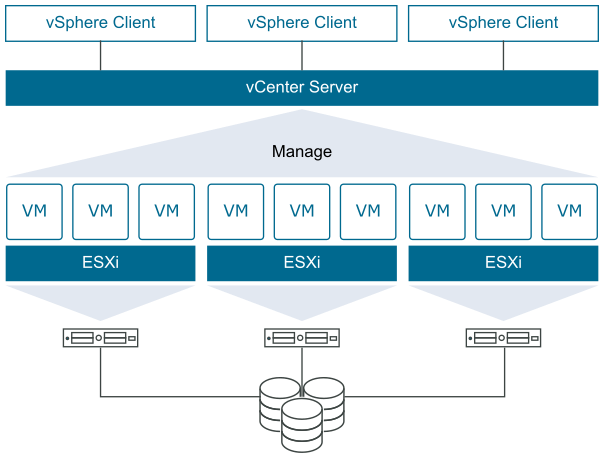
\includegraphics[scale = 0.75]{images/vmware-infrastructure-relationship.png}
    \caption{\href{https://docs.vmware.com/en/VMware-vSphere/index.html}{\textcolor{black}{vSphere's Sotftware Suite Relationship}}}
    \label{VMware}
\end{figure}

\subsection{ESXi}
\href{https://www.vmware.com/products/esxi-and-esx.html}{ESXi} is a type-1, bare-metal hypervisor that is installed directly on a server and functions as the primary operating system. 

Unlike traditional operating systems (e.g., Linux, Windows Server), ESXi focuses solely on allowing virtualization. While traditional operating systems require the installation of a separate software-based type-2 hypervisor for virtualization, ESXi integrates virtualization directly into the operating system itself.

It's important to note that while ESXi enables virtualization at the OS level, the management of virtualization itself is facilitated through VMware's vSphere suite. vSphere provides the tools and features necessary to create, manage, and optimize virtualized environments. It serves as the management layer for the virtualization capabilities enabled by ESXi.

\begin{figure}[H]
    \centering
    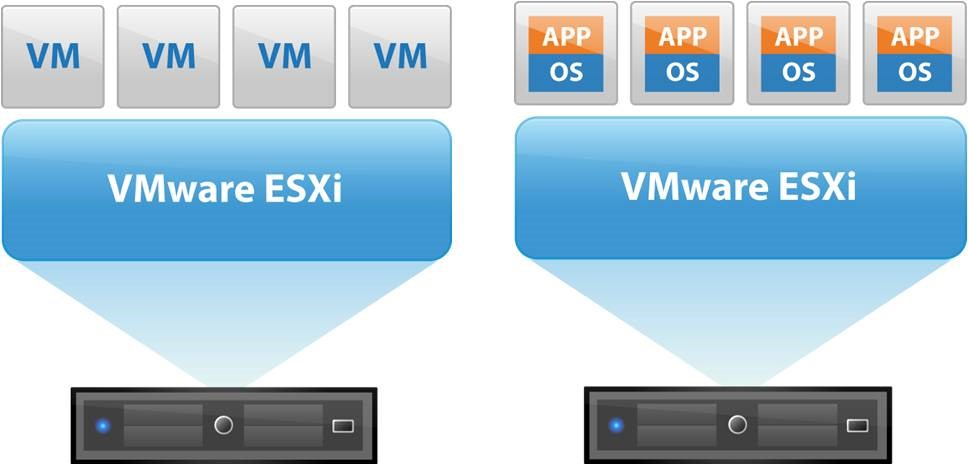
\includegraphics[scale = 0.55]{images/esxi.jpg}
    \caption{\href{https://www.iperiusbackup.net/en/benefits-virtualization-administrator-would-get-from-using-vmware-esxi/}{\textcolor{black}{ESXi}}}
    \label{ESXi}
\end{figure}

\subsection{vSphere Client}
The \href{https://docs.vmware.com/en/VMware-vSphere/7.0/com.vmware.vsphere.vcenterhost.doc/GUID-A618EF76-638A-49DA-991D-B93C5AC0E2B1.html}{vSphere Client} is an application (interface) that allows you to manage and monitor your VMware environments. It is important to note that the actual management capabilities stem from the vCenter Server and \textbf{NOT} from vSphere client.

\begin{figure}[H]
    \centering
    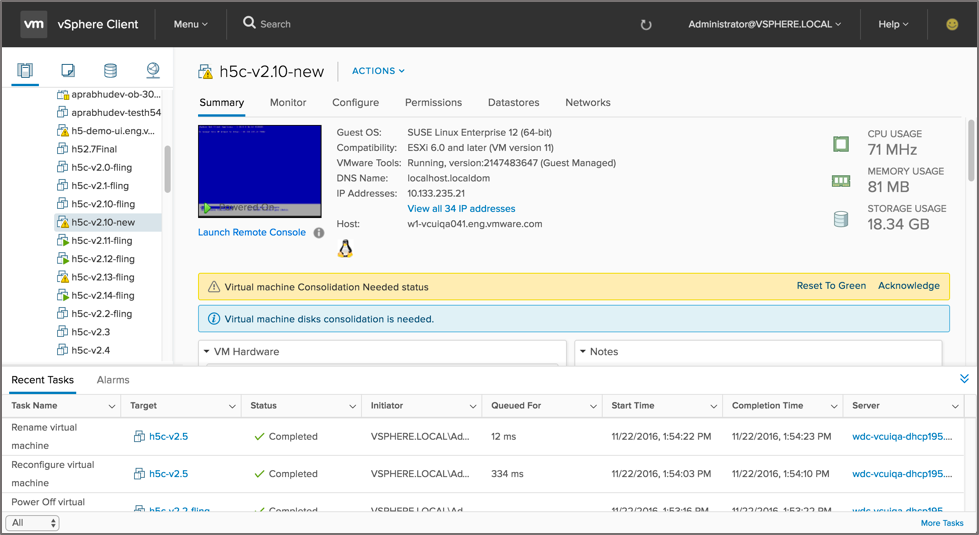
\includegraphics[scale = 0.9]{images/vsphere-client.jpg}
    \caption{\href{https://blogs.vmware.com/vsphere/2016/12/new-vcenter-management-clients-vsphere-6-5.html}{\textcolor{black}{vSphere Client}}}
    \label{vSphere Client}
\end{figure}

\subsection{vCenter}
The vCenter Server is a centralized platform for managing vSphere environments. 

While vSphere serves as the foundation for virtualization, vCenter Server extends these capabilities by acting as a centralized platform designed to manage vSphere environments. Beyond the basic management features offered by vSphere, vCenter Server offers advanced functionalities such as automation, orchestration, and policy-based management.

Some key features of vCenter include: VM migration, security groups, role policies, single sign-on, workflow automation, monitoring and auditing reports, distributed resource management, and optimized resource allocation.

\subsubsection{vCenter Security and Risks}
Security is a critical aspect of virtualized environments, and vCenter provides a range of security features to protect against unauthorized access, data theft, and data manipulation. These security features include: role-based access control\footnote{Define roles and permissions to users based on their roles to prevent unauthorized access.}, auditing\footnote{Track user activity and changes to identify security issues and log actions taken within the virtualized environment.}, encryption\footnote{Encrypt VM data, configuration files, and communication between hosts.}, secure communication\footnote{Supports SSL/TLS encryption to secure communication between hosts and the vCenter server.}, integration\footnote{Integrate with third-party security products (e.g., antivirus, IDS) to provide additional layers of security}, and two-factor authentication\footnote{Provide two forms of identification before accessing the VM to prevent unauthorized access.}. These security features help to ensure confidentiality, integrity, and availability of the virtualized infrastructure, a requirement when working with PHI data. 

\subsection{vSAN}
\href{https://docs.vmware.com/en/VMware-vSphere/7.0/com.vmware.vsphere.vsan-planning.doc/GUID-A80526C8-A941-4F84-9D44-D4B8B3914A95.html}{vSAN} is a software-defined storage solution developed by VMware, which allows organizations to create a distributed storage platform that is integrated with vSphere \cite{VMware3}. This provides a highly scalable and available storage infrastructure, using standard hardware.

By creating a shared data store using the internal disks of ESXi hosts in a vSphere cluster, vSAN allows organizations to pool their storage capacity and performance into a single datastore, scaling it easily by adding more hosts to the cluster. vSAN features data replication, erasure coding, and automatic data rebalancing. Additionally, it offers advanced storage services such as deduplication, compression, and encryption, ensuring optimal storage efficiency and security which streamlines storage management, automates routine tasks, and helps to optimize storage utilization and cost savings.

\begin{figure}[H]
    \centering
    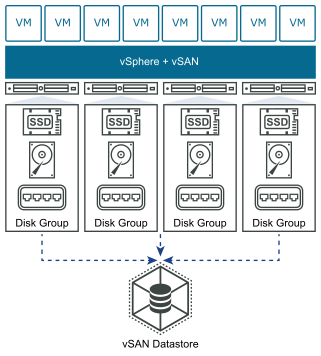
\includegraphics[scale = .8]{images/vsan-deployment.png}
    \caption{\href{https://docs.vmware.com/en/VMware-vSphere/7.0/com.vmware.vsphere.vsan-planning.doc/GUID-A80526C8-A941-4F84-9D44-D4B8B3914A95.html}{\textcolor{black}{Standard vSAN Cluster}}}
    \label{vSan}
\end{figure}

\subsection{NSX}
\href{https://docs.vmware.com/en/VMware-NSX/index.html}{NSX} is a network virtualization and security platform created by VMware that provides a software-defined networking (SDN) solution that enables organizations to virtualize their network infrastructure, creating a more flexible, scalable, and manageable network.

NSX allows for all network components in your infrastructure to be virtualized, decoupling your network from existing hardware. This abstraction enables organizations to pool and automate network resources, which can reduce the time and cost of deploying and managing network infrastructure. NSX also offers advanced security features and networking capabilities which allows administrators to apply precise policies to specific workloads or applications. For example, NSX provides: network automation, multi-cloud and on-premises support, network segmentation, minimal cost and resource overhead, switching and routing, and load balancing features. 

\begin{figure}[H]
    \centering
    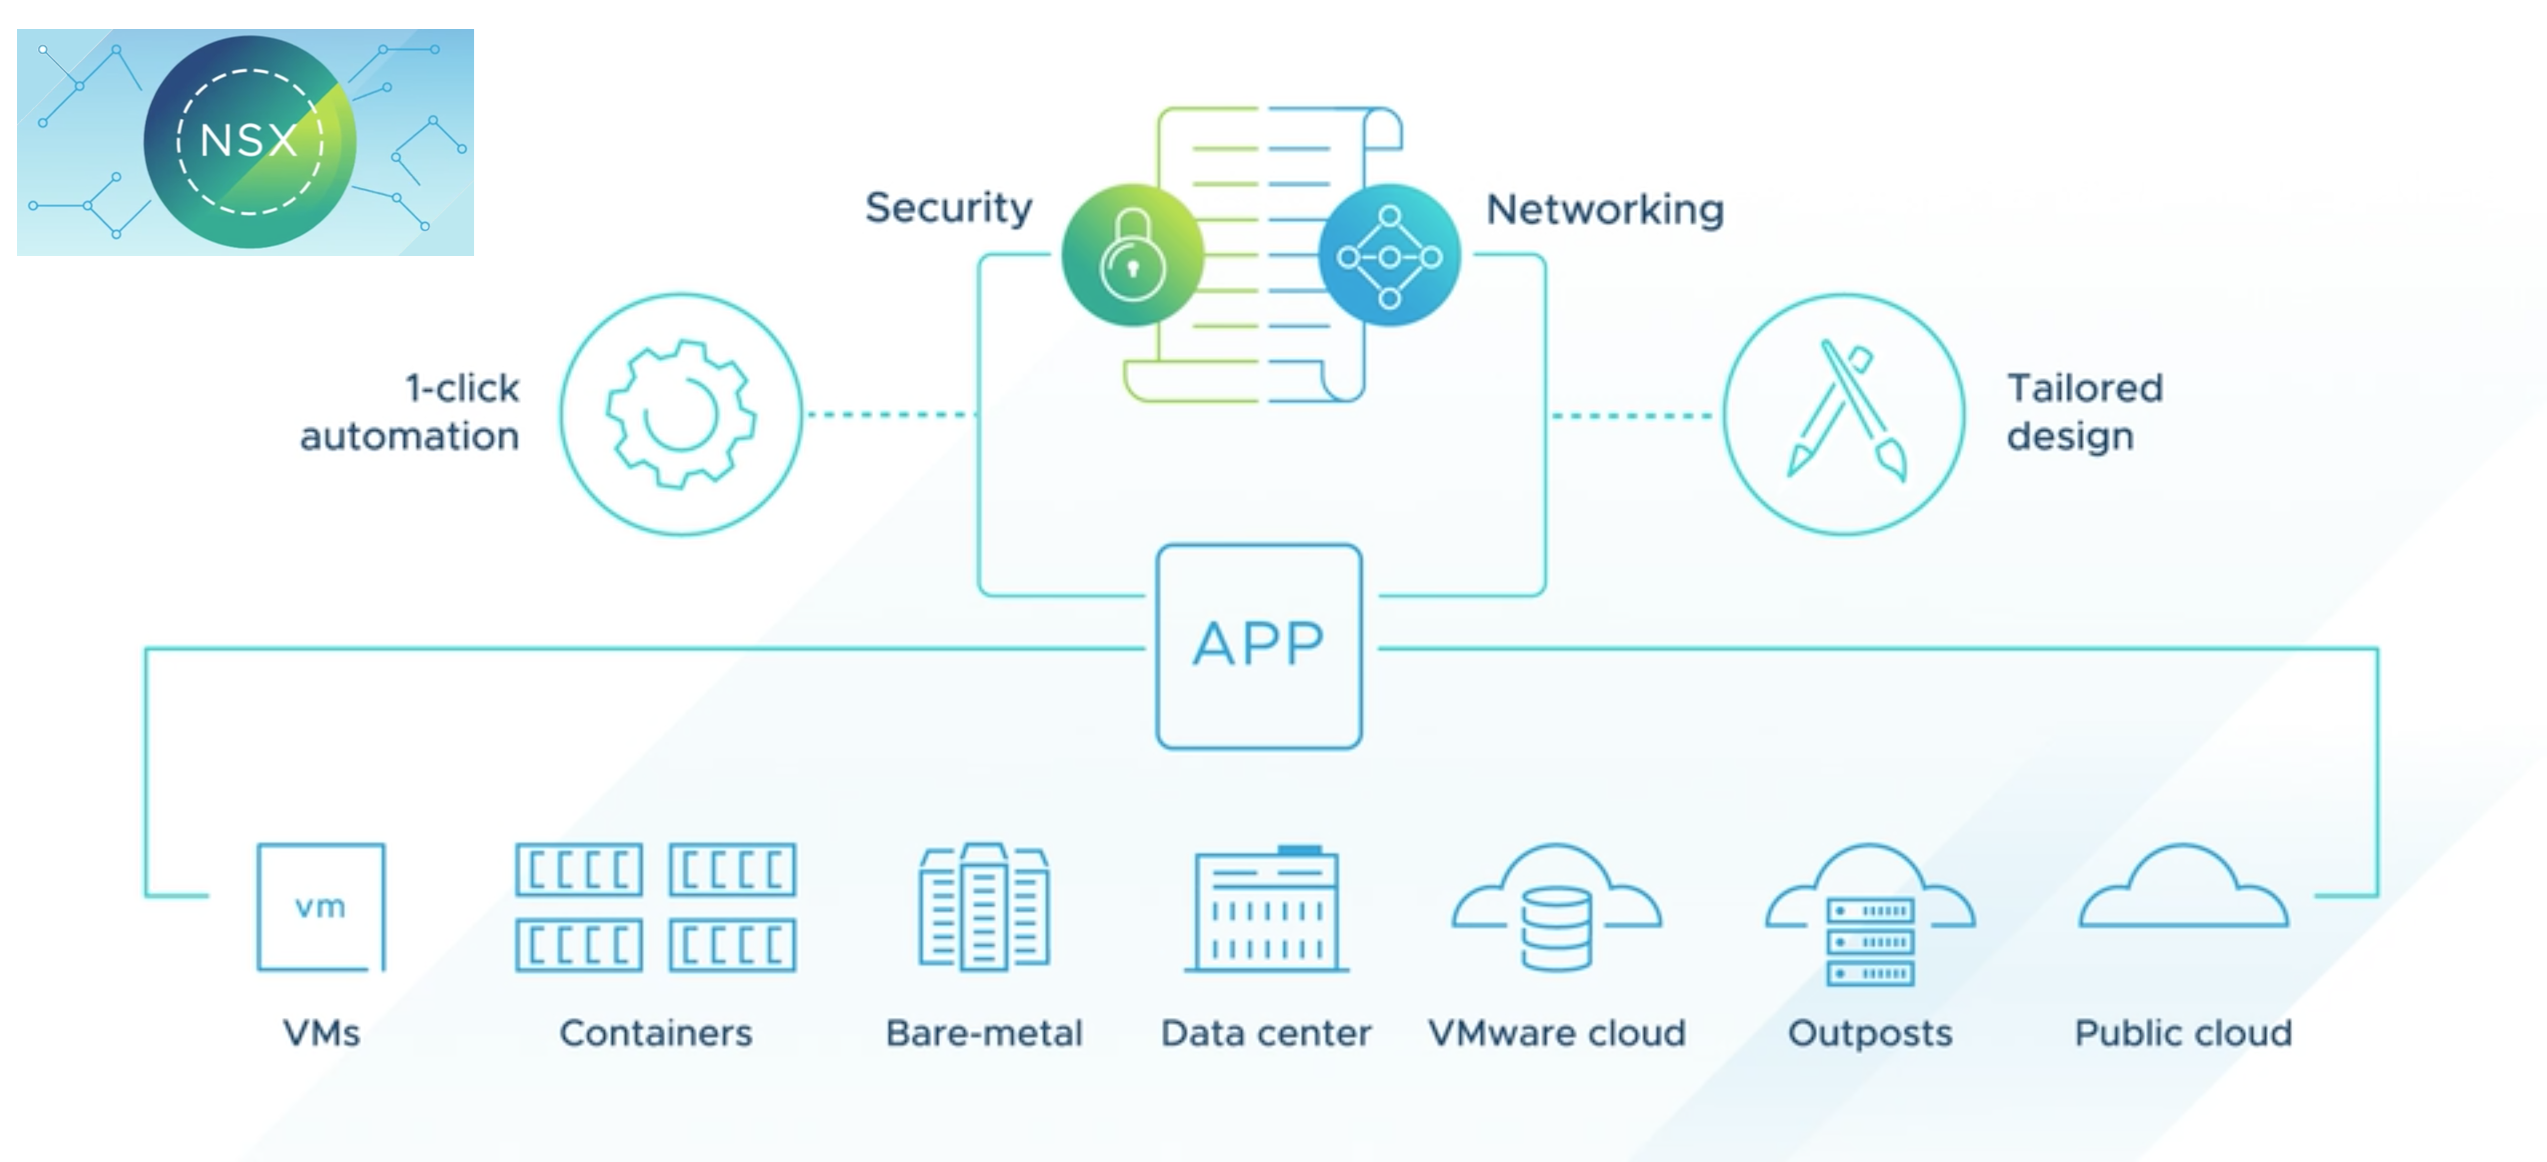
\includegraphics[scale = .19]{images/nsx-diagram.png}
    \caption{\href{https://www.linkedin.com/pulse/vmware-nsxdatacenter-full-stack-solution-part-1-ahmad-karim/}{\textcolor{black}{NSX Infrastructure}}}
    \label{NSX}
\end{figure}

\subsection{VMotion}
\href{https://www.vmware.com/products/vsphere/vmotion.html#:~:text=vMotion%20allows%20you%20to%3A,a%20virtual%20machine%20in%20seconds}{VMotion} is virtualization software that migrates VMs between physical servers or hosts without disrupting service \cite{Murray1}. The process involves copying the entire state of the VM, including memory, CPU state, and network connections, from one host to another. 

To ensure HIPAA compliance when migrating VMs with protected health information (PHI), it is crucial to employ secure protocols and encryption mechanisms to ensure confidentiality, integrity, and availability of PHI during the migration process. IT administrators should utilize encrypted connections or VPN tunnels when transmitting data between the source and destination hosts. By implementing these security measures, host servers and network connections used for VMotion are protected from unauthorized access, mitigating potential compliance issues. 

\begin{figure}[H]
    \centering
    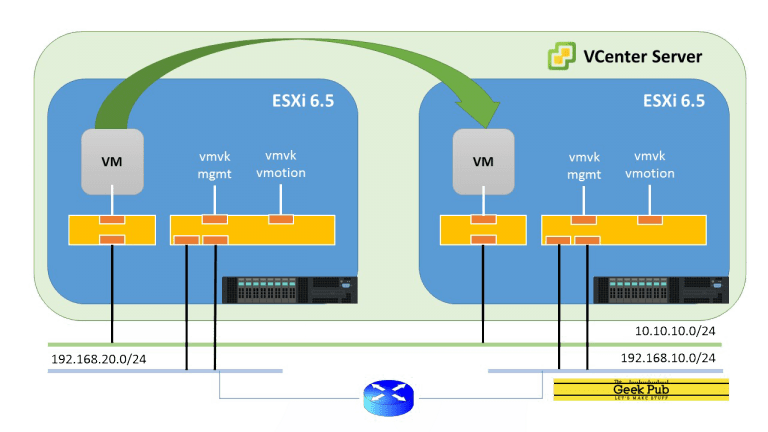
\includegraphics[scale = .50]{images/vmotion.png}
    \caption{\href{https://www.thegeekpub.com/8407/how-vmotion-works/}{\textcolor{black}{VMotion}}}
    \label{VMotion}
\end{figure}